\documentclass{article}
\usepackage{graphicx} % Required for inserting images
\graphicspath{ {./images/} }
\usepackage[square,numbers]{natbib}
\usepackage[letterpaper,top=2cm,bottom=2cm,left=3cm,right=3cm,marginparwidth=1.75cm]{geometry}
\usepackage{hyperref}
\usepackage{placeins}

\bibliographystyle{dinat}


\begin{document}


\title{Unit 13}
\author{Chris Hadden}
\date{}
\maketitle

\section{P5 Social media channels to be used in a digital marketing campaign}

We have been asked to develop a social media campaign for a local pet shop, Pampered Pets.
They have set themselves up in direct competition with Pets at Home but they are a family run business and so really care about their customers. 
They sell everything pets need, but they take an ethical stand on not selling animals. 
They want to make the most of the profitable Spring / Summer trade and make sure that pet treats and care pack for new pets bought from themselves will lead to ongoing online sales.

We have produced this report to explain what channels Pampered Pets will need to use as a part of their digital marketing campaign.
We also outline our plans for the content of that campaign.

\bigskip

\subsection{Narrowing our focus}
There is a plethora of different types of social media channels, never mind specific social media sites.
As our client are an independent business, they do not have the money or staff to be able to cover every type of social media. Because of this we are going to have to consider where they will be able to make the largest impact from the smallest outlay.

To narrow down the list of channels we will concentrate on the main points we need to consider, which are:
\begin{itemize}
    \item How often does the client want to publish updates
    \item Which channels are popular
    \item What does the client want to get out of a campaign
\end{itemize}

\newpage
\subsection{What channels are popular}
As we can see from the SproutSocial, a social media management firm, in figure \ref{fig:pie}\cite{sprout} that consumers much prefer social media over other forms of contact with brands
\FloatBarrier
\begin{figure}[ht]
    \caption{Pie graph of preferred brand contact}
    \centering
    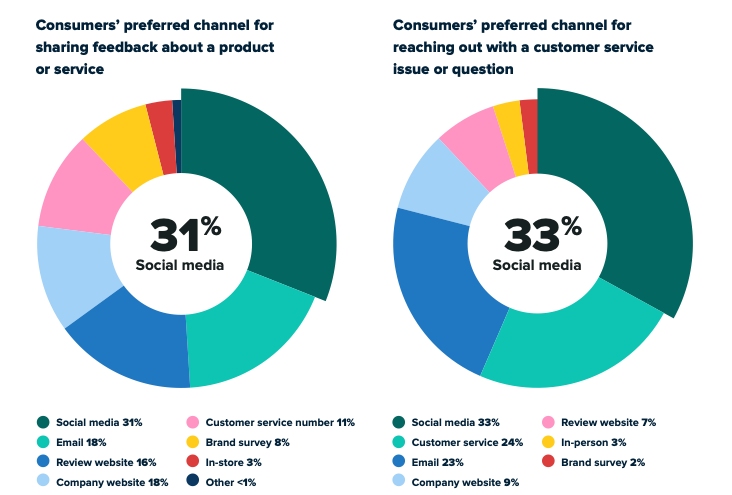
\includegraphics[width=0.8\textwidth]{sprout-index-consumers}
    \label{fig:pie}
    \end{figure}
    \FloatBarrier

At the very least we can say that social media is the right place to start.
\subsubsection{What does the client want to get out of a campaign}
According to the site SproutSocial, they found that for marketing "88\% of marketers report that their social media strategy positively influenced their sales and 90\% agree that social media helps them stay ahead of their competitors."\cite{sprout}. Having talked to Pampered Pets, what they said they wanted to get out of their campaign was increased online sales over Spring / Summer and the SproutSocial report would seem to indicate that a social media campaign could deliver what they wanted.


\newpage
\subsubsection{How often does Pampered Pets want to post}
Pampered Pets are a small company with no dedicated social media manager, or the money to pay for a 3rd party to take on that work. 
This means that they really only have the capacity to post at most every day or so with new offers, etc. 
\begin{figure}[ht]
    \caption{When to share}
    \centering
    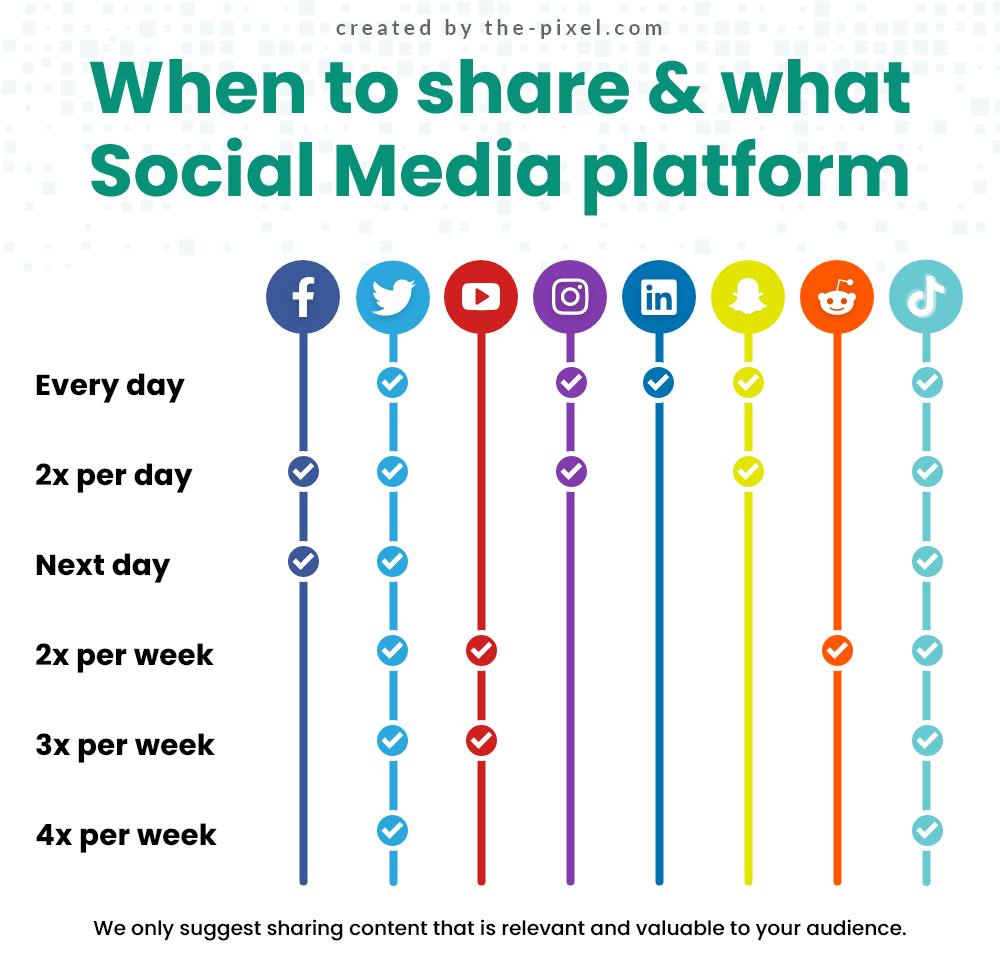
\includegraphics[width=0.8\textwidth]{sharing-on-social-media-channels}
    \label{fig:days}
    \end{figure}
    \FloatBarrier
 As figure \ref{fig:days} from Pixel \cite{pixel} shows, posting at this rate would seem to indicate that the likes of Facebook, Twitter (X) or Instagram may be good matches.

 \section{Conclusion}
 It would seem that the channel with the greatest impact and the channel that most consumers actually want to use is social media. We have identified a numer of possible platforms that would be good for Pampered Pets to make a presence on. From this we will need to further delve in to who Pampered Pets should be targeting.

\bibliography{bibliography}

\end{document}

